\chapter{Continuité et Limites}

\section{Rappels Théoriques}

\subsection{Continuité}
\begin{definition}[Continuité en un point]
Une fonction $f$ définie sur un intervalle ouvert contenant $x_0$ est continue en $x_0$ si :
\[ \lim_{x \to x_0} f(x) = f(x_0) \]
\end{definition}

\begin{propriete}
\begin{itemize}
    \item Les fonctions polynômes, sinus, cosinus sont continues sur $\mathbb{R}$.
    \item Les fonctions rationnelles sont continues sur leur domaine de définition.
    \item La somme, le produit et la composée de fonctions continues sont des fonctions continues.
\end{itemize}
\end{propriete}

\subsection{Théorème des Valeurs Intermédiaires (TVI)}
Ce théorème est fondamental pour prouver l'existence de solutions d'équations du type $f(x) = k$.

\begin{center}
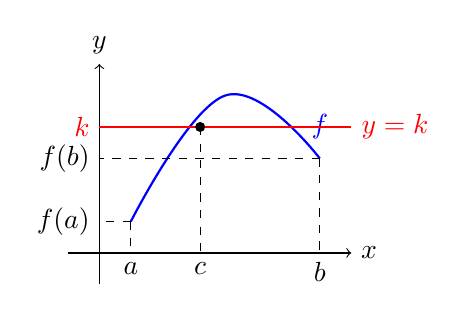
\begin{tikzpicture}[scale=0.8]
    % Axes
    \draw[->] (-0.5,0) -- (4,0) node[right] {$x$};
    \draw[->] (0,-0.5) -- (0,3) node[above] {$y$};
    
    % Fonction
    \draw[thick, blue] plot [smooth, tension=0.7] coordinates {(0.5,0.5) (2,2.5) (3.5,1.5)};
    \node[blue] at (3.5,2) {$f$};
    
    % Points a et b
    \draw[dashed] (0.5,0.5) -- (0.5,0) node[below] {$a$};
    \draw[dashed] (0.5,0.5) -- (0,0.5) node[left] {$f(a)$};
    \draw[dashed] (3.5,1.5) -- (3.5,0) node[below] {$b$};
    \draw[dashed] (3.5,1.5) -- (0,1.5) node[left] {$f(b)$};
    
    % Valeur k
    \draw[red, thick] (0,2) -- (4,2) node[right] {$y=k$};
    \node[left, red] at (0,2) {$k$};
    
    % Intersection
    \draw[dashed] (1.6,2) -- (1.6,0) node[below] {$c$};
    \filldraw (1.6,2) circle (2pt);
\end{tikzpicture}
\end{center}

\begin{theoreme}[TVI Général]
Si $f$ est continue sur un intervalle $[a, b]$ et si $k$ est un réel compris entre $f(a)$ et $f(b)$, alors l'équation $f(x) = k$ admet \textbf{au moins une solution} $\alpha$ dans $[a, b]$.
\end{theoreme}

\begin{theoreme}[TVI et Stricte Monotonie - Théorème de la Bijection]
Si $f$ est continue \textbf{et strictement monotone} sur un intervalle $I$ (borné ou non), alors $f$ réalise une bijection de $I$ sur $J = f(I)$.
Pour tout $k \in J$, l'équation $f(x) = k$ admet une \textbf{unique solution} $\alpha$ dans $I$.
\end{theoreme}

\subsection{Limites et Branches Infinies}
Soit $f$ une fonction et $\mathcal{C}_f$ sa courbe représentative.

\begin{itemize}
    \item \textbf{Asymptote Verticale :} Si $\lim_{x \to a} f(x) = \pm \infty$, alors la droite d'équation $x = a$ est asymptote verticale à $\mathcal{C}_f$.
    \item \textbf{Asymptote Horizontale :} Si $\lim_{x \to \pm \infty} f(x) = L$ ($L \in \mathbb{R}$), alors la droite d'équation $y = L$ est asymptote horizontale en $\pm \infty$.
    \item \textbf{Asymptote Oblique :} La droite $\Delta: y = ax + b$ est asymptote oblique en $+\infty$ si $\lim_{x \to +\infty} [f(x) - (ax+b)] = 0$.
    
    \textbf{Méthode pratique :}
    \begin{enumerate}
        \item Calculer $\lim_{x \to \infty} \frac{f(x)}{x} = a$.
        \item Si $a \in \mathbb{R}^*$, calculer $\lim_{x \to \infty} [f(x) - ax] = b$.
        \item Si $b \in \mathbb{R}$, alors $y = ax + b$ est asymptote oblique.
    \end{enumerate}
    
    \item \textbf{Branches Paraboliques :}
    \begin{itemize}
        \item Si $\lim \frac{f(x)}{x} = 0$, branche parabolique de direction $(Ox)$.
        \item Si $\lim \frac{f(x)}{x} = \pm \infty$, branche parabolique de direction $(Oy)$.
        \item Si $\lim \frac{f(x)}{x} = a \neq 0$ et $\lim [f(x) - ax] = \pm \infty$, branche parabolique de direction asymptotique $y=ax$.
    \end{itemize}
\end{itemize}

\subsection{Limite d'une fonction composée}
Soient $f$ et $g$ deux fonctions.
\begin{theoreme}
Si $\lim_{x \to x_0} g(x) = L$ et si la fonction $f$ est \textbf{continue en $L$}, alors :
\[ \lim_{x \to x_0} f(g(x)) = f(L) \]
\end{theoreme}
\begin{remarque}
Si $\lim_{x \to x_0} g(x) = L$ et $\lim_{X \to L} f(X) = \ell$ (où $L$ et $\ell$ peuvent être finis ou infinis), alors $\lim_{x \to x_0} f(g(x)) = \ell$.
Cependant, pour appliquer la formule directe $f(\lim g(x))$, la continuité de $f$ est requise.
\end{remarque}

\section{Exercices de Compréhension}

\begin{rappel}
\textbf{Objectif :} Maîtriser les définitions de base et les calculs de limites simples.
\end{rappel}

\textbf{Exercice 1.1 : Continuité} \\
Soit la fonction $f$ définie sur $\mathbb{R}$ par :
\[ f(x) = \begin{cases} \frac{x^2 - 1}{x - 1} & \text{si } x \neq 1 \\ 2 & \text{si } x = 1 \end{cases} \]
Étudier la continuité de $f$ en 1.

\begin{correction}
Pour $x \neq 1$, $f(x) = \frac{(x-1)(x+1)}{x-1} = x+1$. \\
Calculons la limite en 1 : $\lim_{x \to 1} f(x) = \lim_{x \to 1} (x+1) = 2$. \\
Or, $f(1) = 2$. \\
Comme $\lim_{x \to 1} f(x) = f(1)$, \textbf{la fonction $f$ est continue en 1}.
\end{correction}

\textbf{Exercice 1.2 : TVI} \\
Montrer que l'équation $x^3 + 2x - 1 = 0$ admet une unique solution $\alpha$ dans l'intervalle $[0, 1]$.

\begin{correction}
Soit $g(x) = x^3 + 2x - 1$.
\begin{enumerate}
    \item $g$ est une fonction polynôme, donc \textbf{continue} sur $\mathbb{R}$ et en particulier sur $[0, 1]$.
    \item $g'(x) = 3x^2 + 2$. Pour tout $x \in \mathbb{R}$, $g'(x) > 0$. Donc $g$ est \textbf{strictement croissante} sur $[0, 1]$.
    \item $g(0) = -1$ et $g(1) = 2$.
    \item On constate que $0 \in [-1, 2]$ (ou que $g(0) \times g(1) < 0$).
\end{enumerate}
D'après le théorème de la bijection (ou TVI strict), l'équation $g(x) = 0$ admet une \textbf{unique solution} $\alpha \in [0, 1]$.
\end{correction}

\textbf{Exercice 1.3 : Calcul de Limites (Formes Indéterminées)} \\
Calculer les limites suivantes :
\begin{enumerate}
    \item $\lim_{x \to +\infty} \sqrt{x^2+1} - x$
    \item $\lim_{x \to 0} \frac{\sin(3x)}{\sqrt{1+x}-1}$
\end{enumerate}

\begin{correction}
\textbf{1. Expression conjuguée}
Forme indéterminée "$\infty - \infty$".
\[ \sqrt{x^2+1} - x = \frac{(\sqrt{x^2+1}-x)(\sqrt{x^2+1}+x)}{\sqrt{x^2+1}+x} = \frac{(x^2+1)-x^2}{\sqrt{x^2+1}+x} = \frac{1}{\sqrt{x^2+1}+x} \]
$\lim_{x \to +\infty} \sqrt{x^2+1}+x = +\infty$, donc $\lim_{x \to +\infty} f(x) = 0$.

\textbf{2. Limite trigonométrique et taux d'accroissement}
Forme "0/0".
\[ \frac{\sin(3x)}{\sqrt{1+x}-1} = \frac{\sin(3x)}{3x} \times 3 \times \frac{1}{\frac{\sqrt{1+x}-1}{x}} \]
Or $\lim_{x \to 0} \frac{\sin(3x)}{3x} = 1$.
Et $\lim_{x \to 0} \frac{\sqrt{1+x}-1}{x} = \lim_{x \to 0} \frac{1}{\sqrt{1+x}+1} = \frac{1}{2}$ (ou par dérivée de $\sqrt{1+x}$ en 0).
Donc Limite $= 1 \times 3 \times \frac{1}{1/2} = 6$.
\end{correction}

\textbf{Exercice 1.4 : Vrai ou Faux ?}
Répondre par Vrai ou Faux en justifiant.
\begin{enumerate}
    \item Si $f$ est continue en $x_0$, alors $|f|$ est continue en $x_0$.
    \item Si $\lim_{x \to +\infty} f(x) = +\infty$ et $\lim_{x \to +\infty} g(x) = -\infty$, alors $\lim_{x \to +\infty} (f(x)+g(x)) = 0$.
\end{enumerate}

\begin{correction}
\begin{enumerate}
    \item \textbf{Vrai.} La fonction valeur absolue est continue sur $\mathbb{R}$. La composée de fonctions continues est continue.
    \item \textbf{Faux.} C'est une forme indéterminée "$\infty - \infty$". Contre-exemple : $f(x)=x^2$ et $g(x)=-x$. Somme $\to +\infty$.
\end{enumerate}
\end{correction}

\autoeval{

\begin{exobac}
\textbf{Sujet : Étude de fonction, continuité et bijection.}

Soit la fonction $f$ définie sur $I = [0, +\infty[$ par $f(x) = \sqrt{x} e^{1-x}$.
\begin{enumerate}
    \item Étudier la continuité et la dérivabilité de $f$ sur $I$. Préciser la dérivabilité en 0.
    \item Dresser le tableau de variation de $f$.
    \item Montrer que l'équation $f(x) = 1$ admet exactement deux solutions dont l'une est 1.
    \item Soit $g$ la restriction de $f$ à l'intervalle $[1, +\infty[$. Montrer que $g$ admet une fonction réciproque $g^{-1}$ définie sur un intervalle $J$ que l'on précisera.
\end{enumerate}
\end{exobac}

\begin{correction}
\textbf{1. Continuité et Dérivabilité}
\begin{itemize}
    \item $x \mapsto \sqrt{x}$ est continue sur $[0, +\infty[$ et dérivable sur $]0, +\infty[$.
    \item $x \mapsto e^{1-x}$ est continue et dérivable sur $\mathbb{R}$.
    \item Par produit, $f$ est \textbf{continue sur $[0, +\infty[$} et \textbf{dérivable sur $]0, +\infty[$}.
\end{itemize}
\textbf{Dérivabilité en 0 :}
\[ \lim_{x \to 0^+} \frac{f(x) - f(0)}{x - 0} = \lim_{x \to 0^+} \frac{\sqrt{x}e^{1-x}}{x} = \lim_{x \to 0^+} \frac{e^{1-x}}{\sqrt{x}} \]
Quand $x \to 0^+$, $\sqrt{x} \to 0^+$ et $e^{1-x} \to e$. Donc la limite est $+\infty$.
$f$ n'est \textbf{pas dérivable en 0}. La courbe $\mathcal{C}_f$ admet une demi-tangente verticale au point d'abscisse 0.

\textbf{2. Variations}
Pour $x > 0$, calculons $f'(x)$ :
\[ f'(x) = (\frac{1}{2\sqrt{x}})e^{1-x} + \sqrt{x}(-e^{1-x}) = e^{1-x} \left( \frac{1}{2\sqrt{x}} - \sqrt{x} \right) = e^{1-x} \left( \frac{1 - 2x}{2\sqrt{x}} \right) \]
Le signe de $f'(x)$ dépend du signe de $1 - 2x$.
\begin{itemize}
    \item $f'(x) > 0$ pour $x \in ]0, 1/2[$.
    \item $f'(x) < 0$ pour $x \in ]1/2, +\infty[$.
    \item $f'(x) = 0$ pour $x = 1/2$.
\end{itemize}
\textbf{Tableau de variation :}
$f$ est croissante sur $[0, 1/2]$ et décroissante sur $[1/2, +\infty[$.
Maximum en $1/2$ : $f(1/2) = \sqrt{1/2}e^{1/2} = \frac{\sqrt{2}}{2}\sqrt{e} \approx 1.16$.
Limite en $+\infty$ : $\lim_{x \to +\infty} \sqrt{x}e^{1-x} = \lim_{x \to +\infty} \frac{e}{\frac{e^x}{\sqrt{x}}} = 0$ (croissance comparée).

\textbf{3. Équation $f(x) = 1$}
\begin{itemize}
    \item Sur $[0, 1/2]$, $f$ est continue et strictement croissante. $f(0)=0$ et $f(1/2) \approx 1.16$. Comme $1 \in [0, f(1/2)]$, il existe une unique solution $\alpha_1$.
    \item Sur $[1/2, +\infty[$, $f$ est continue et strictement décroissante. $f(1/2) \approx 1.16$ et $\lim_{+\infty} f = 0$. Comme $1 \in ]0, f(1/2)]$, il existe une unique solution $\alpha_2$.
    \item Vérifions pour $x=1$ : $f(1) = \sqrt{1}e^{1-1} = 1 \cdot e^0 = 1$. Donc \textbf{1 est bien une solution}.
\end{itemize}
Conclusion : L'équation admet exactement deux solutions.

\textbf{4. Bijection réciproque}
$g$ est la restriction de $f$ à $[1, +\infty[$.
Sur cet intervalle, $g$ est \textbf{continue} et \textbf{strictement décroissante}.
Elle réalise donc une bijection de $[1, +\infty[$ sur $J = g([1, +\infty[) = ]\lim_{+\infty}g, g(1)] = ]0, 1]$.
$g^{-1}$ est définie sur $J = ]0, 1]$.
\end{correction}

\autoeval{
Je sais lever une indétermination "$\infty - \infty$" (conjugué, factorisation) & & \\ \hline
Je connais le TVI et ses conditions d'application & & \\ \hline
Je sais étudier la continuité d'une fonction définie par morceaux & & \\ \hline
Je sais trouver une asymptote oblique & & \\
}

\section{Exercices Type Bac}
